\documentclass[border=5pt]{standalone}
\usepackage{tikz}
\usepackage{amsmath}
\usetikzlibrary{patterns, positioning}

\begin{document}

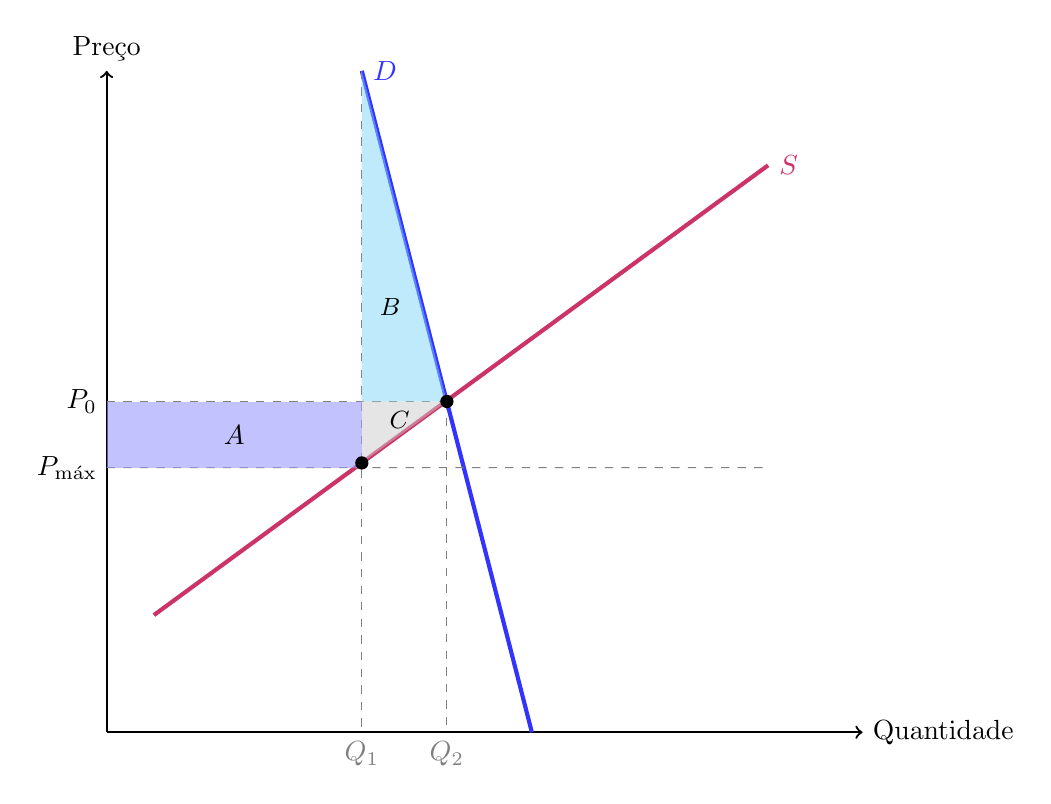
\begin{tikzpicture}[scale=1.2]
    % Eixos
    \draw[thick, ->] (0,0) -- (8,0) node[right] {Quantidade};
    \draw[thick, ->] (0,0) -- (0,7) node[above] {Preço};
    
    % Curva de Demanda (D) - mais vertical (inelástica), passa por (3.6, 3.5) e (4.5, 0)
    % y = 17.5 - 3.89*x, em y=7: x = (17.5-7)/3.89 = 2.7
    \draw[thick, blue!80, line width=1.5pt] (2.7,7) node[right] {$D$} -- (4.5,0);
    
    % Curva de Oferta (S) - passa por (3.6, 3.5)
    % Ajustando para interceptar exatamente em (3.6, 3.5)
    \draw[thick, purple!80, line width=1.5pt] (0.5,1.24) -- (7,6.0) node[right] {$S$};
    
    % Interseção (equilíbrio de mercado) em Q2, P0
    \coordinate (E) at (3.6,3.5);
    
    % Preço de equilíbrio
    \coordinate (P0) at (0,3.5);
    \draw[dashed, gray] (P0) -- (E);
    \draw (0,3.5) node[left] {$P_0$};
    
    % Preço máximo
    \coordinate (Pmax) at (0,2.8);
    \draw[dashed, gray] (Pmax) -- (7,2.8);
    \draw (0,2.8) node[left] {$P_{\text{máx}}$};
    
    % Quantidades
    \draw[dashed, gray] (2.7,7) -- (2.7,0) node[below] {$Q_1$};
    \draw[dashed, gray] (3.6,3.5) -- (3.6,0) node[below] {$Q_2$};
    
    % Pontos de interseção
    % Oferta em x=2.7: y = 1.24 + (6.0-1.24)/(7-0.5) * (2.7-0.5) = 2.85
    \coordinate (S1) at (2.7,2.85);
    \coordinate (D1) at (3.45,2.8);
    
    % Área A (retângulo - excedente transferido)
    \fill[blue!40, opacity=0.6] (0,2.8) rectangle (2.7,3.5);
    \node at (1.35,3.15) {$A$};
    
    % Área B (triângulo - abaixo da curva de demanda até P0)
    % Pontos: (2.7, P_max=2.8), (2.7, P0=3.5), ponto na demanda em x=2.7 (que é y=7, mas limitado por P0)
    % Na verdade: de Q1 até Q2, abaixo da demanda e acima de P0
    \fill[cyan!50, opacity=0.5] (2.7,3.5) -- (3.6,3.5) -- (2.7,7) -- cycle;
    \node at (3.0,4.5) {\small $B$};
    
    % Área C (triângulo - acima da curva de oferta e abaixo de P0)
    % Pontos: (2.7, oferta em 2.7=2.85), (2.7, P0=3.5), (3.6, P0=3.5)
    \fill[gray!40, opacity=0.5] (2.7,2.85) -- (2.7,3.5) -- (3.6,3.5) -- cycle;
    \node at (3.1,3.3) {\small $C$};
    
    % Pontos principais
    \fill (E) circle (2pt);
    \fill (S1) circle (2pt);

\end{tikzpicture}

\end{document}
